\section{Experiments}
\begin{frame}
	\frametitle{Experiments}
	\tableofcontents[currentsection]
\end{frame}

\subsection{Method}
\begin{frame}{Experiments}{Method}		
	\begin{columns}
		\begin{column}{0.5\textwidth}
			\begin{itemize}
				\item Design set-up
				\item Control and adjust equipment
				\item Perform the experiment
			\end{itemize}	
		\end{column}
		\begin{column}{0.5\textwidth} 
			\begin{equation*}
			H(f)=\frac{Y(f)}{X(f)}=\frac{\mathscr{F}(y(t))\times\mathscr{F}^{\ast}(x(t))}{\mathscr{F}(x(t))\times\mathscr{F}^{\ast}(x(t))}
		\end{equation*}
		\end{column}
	\end{columns}
\end{frame}

\begin{frame}{Experiments}{Control and Adjusting}		
	\begin{columns}
		\begin{column}{0.5\textwidth}
			\begin{itemize}
				\item Using a reference calibrator
				\item Yields a given dB @ calibrators frequency
				\item Record and examine signal
				\item Account for the difference 
			\end{itemize}	
		\end{column}	
		\begin{column}{0.5\textwidth} 
		\end{column}
	\end{columns}
\end{frame}

\subsection{Listening Test}
\begin{frame}{Experiments}{Listening Test}		
	\begin{columns}
		\begin{column}{0.5\textwidth}
			\begin{itemize}
				\item Determining threshold
				\item Using AAU students
				\item Results
				\begin{itemize}
					\item 10 dB attenuation is required
				\end{itemize}
			\end{itemize}	
		\end{column}	
		\begin{column}{0.5\textwidth} 
			\begin{figure}
					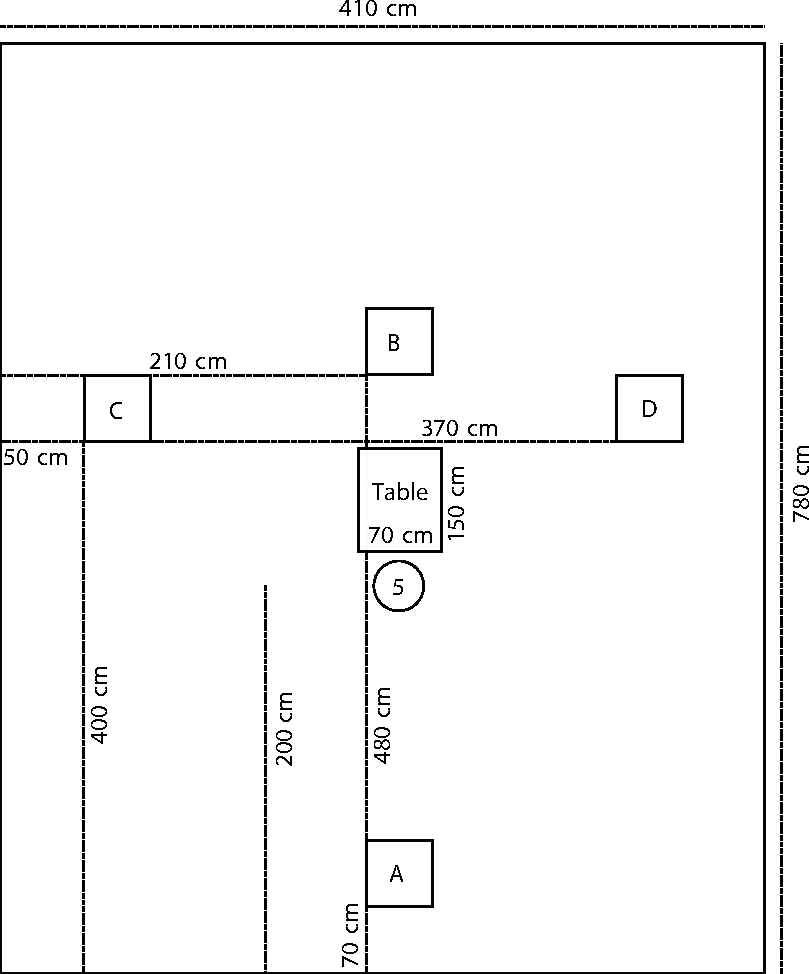
\includegraphics[width=1\textwidth]{figures/ListeningTestSetup.jpg}
			\end{figure}
		\end{column}
	\end{columns}
\end{frame}

\subsection{Measuring a Transfer-Function}
\begin{frame}{Experiments}{Measuring a Transfer-Function (Headphone)}		
	\begin{columns}
		\begin{column}{0.5\textwidth}
			\begin{itemize}
				\item Headphone Transfer-function
				\begin{itemize}
					\item Physical cup of headphone
				\end{itemize}
				\item{Logarithmic Chirp}
			\end{itemize}
		\end{column}
		\begin{column}{0.5\textwidth} 
			\begin{figure}[h]
				\includegraphics[width=1\textwidth]{figures/TransferFunctionHP}
			\end{figure}
		\end{column}
	\end{columns}
\end{frame}

\begin{frame}{Experiments}{Measuring a Transfer-Function (Cancellation Path)}		
	\begin{columns}
		\begin{column}{0.5\textwidth}
			\begin{itemize}
				\item Calcellation Path Transfer-function
				\begin{itemize}
					\item Headphone speaker \\ $\rightarrow$ Error microphone
				\end{itemize}
				\item{Logarithmic Chirp}
			\end{itemize}
		\end{column}
		\begin{column}{0.5\textwidth} 
			\begin{figure}[h]
				\includegraphics[width=1\textwidth]{figures/TransferFunctionCP}
			\end{figure}
		\end{column}
	\end{columns}
\end{frame}

\subsection{Testing the ANC of Other Brand Headphones}
\begin{frame}{Experiments}{Testing Consumer ANC}		
	\begin{columns}
		\begin{column}{0.5\textwidth}
			\begin{itemize}
				\item Tested four consumer headphones
					\begin{itemize}
						\item Tested with and without ANC enabled
						\item Each headphone tested five times
						\item Using the Archimedes project
					\end{itemize}
				\item Using filter-bank to analyze results
				\begin{itemize}
					\item Fourier Transform only works on LTI-systems
				\end{itemize}
			\end{itemize}
		\end{column}
		\begin{column}{0.5\textwidth} 				
			\begin{figure}[h]
				\includegraphics[width=1\textwidth]{figures/OtherBrandsSetupSide.jpg}
			\end{figure}
		\end{column}
	\end{columns}
\end{frame}










